\documentclass[12pt]{article}
\usepackage[left=2cm,right=2cm,top=3cm,head=4cm,bottom=2cm,a4paper]{geometry}
\usepackage{hyperref}
\usepackage{amsmath}

\usepackage{tikz}
\usetikzlibrary{shadows,arrows.meta,positioning,calc,patterns, shapes}
\definecolor{darkgreen}{RGB}{27,114,30}

\parindent 0pt
\parskip 5pt

\begin{document}
\section{Motivation}

In order to use the extracted cosmics rays to determine the particle flux on Gaia's CCDs, we need to count the cosmics in each observation and additionally need to know the exposed CCD area $A_\mathrm{exp}$ and the CCD exposure time $T_\mathrm{exp}$ for each observation. The flux is then simply computed as

\begin{equation}
  F_\mathrm{cosmics} = \frac{\mathrm{Counts}}{A_\mathrm{exp} \cdot T_\mathrm{exp}}
\end{equation}

In the following, we determine these values for SM-SIF and BAM observations, whose computation are not trivial due to the use of TDI (and in the latter case, staring) observations and the size of the used AL readout windows relative to the physical CCD size.

For our calculations: A Gaia CCD is segmented into 4500 pixels in AL direction and 1980 pixels in AC direction - of these, 14 pixels are in the pre-scan region and not used. Pixels are $10 \times 30\, \mathrm{\mu m}$ (AL x AC) and TDI transfer time is $T_\mathrm{TDI} = 0.9828\, \mathrm{ms/pixel}$, so the effective CCD exposure time is 4.4226\,s.

\section{SM}

The readout of the SM-SIF images are a continuous readout of the signal acquired from TDI (see also Fig. \ref{fig:SM_Acq}). To avoid saturation from bright stars, Gate 12 is permanently activated, leading to a readout of only the last 2900 CCD lines in AL. Pixels are then binned to a factor of 2 in both AL and AC.

\begin{figure}[h]
  \centering
  \begin{tikzpicture}[scale=1]

    % Part 1: A physical image of the CCD, with gate 12
    \node(scope1){
      \begin{tikzpicture} 
        \draw[thick] (0,0) rectangle (1.5,3); % box
        \draw[thick,blue] (0.53,-0.2) -- (0.53,3.2); % Line for gate 12
        \draw[thick,red] (1.5,0) -- (1.5,3); % Readout
        \draw[thick,-{Latex[length=8pt]}] (0.6,1.5) to (1.4,1.5);
        
        \node[blue] at (0.3,3.4) {Gate 12}; % Marker for gate 12
        \node[red] at (1.8,-0.3) {Readout}; % Marker for Readout
        \node at (1,1.8) {TDI}; % Marker for Readout


      \end{tikzpicture} 
    };

    % Part 2: The output image
    \node[at={($(scope1.east)+(.1cm,0)$)},anchor=west](scope2){
      
\begin{tikzpicture} 
        % the box around it
        \draw[thick, fill] (0,0) rectangle (5,3);

        % A few stars
        \node[star,star points=4, star point height=.7cm, draw, fill=white] at (1,1) {};
        \node[star,star points=4, star point height=.1cm, draw, fill=white] at (4,2) {};
        \node[star,star points=4, star point height=.1cm, draw, fill=white] at (.5,2.5) {};

        % And some cosmics
        \draw[thick,white] (3.5,2) -- (3,1.5) (1.2,2.5) -- (1.3,2)
                           (4,0.2) -- (4.5,0.3);
      \end{tikzpicture} 
    };

    % a big arrow between them
    \draw[red, ultra thick,-{Stealth[length=.5cm, width=.7cm]}] ($(scope1.east) + (-1cm,0)$)  to ($(scope2.west)$);

  \end{tikzpicture}
  \caption{Scheme of an SM acquisition. The CCD area of each chip after Gate 12 is continuously read out via TDI (left). The resulting image (right) has the same dimension in AC but a dimension in AL dependent on the duration of the readout.}
  \label{fig:SM_Acq}
\end{figure}



For clarity in notation, I will, from now on, use the following terms:
\begin{itemize}
  \item A \textbf{CCD pixel} refers to a physical pixel on the actual CCD - i.e. one physical unit of $10 \times 30\, \mathrm{\mu m}$
  \item An \textbf{image pixel} refers to a pixel in the image recorded after the TDI scan. While it still carries spatial information in AC, its AL information is a result of the integration over the sampled region in AL - it encodes time and location. Thus, an image pixel does not correspond to a single physical pixel, but rather the history of an entire AL line during TDI.
\end{itemize}


The resulting image, then, consists of 983 image pixels in AC and a variable number $N_\mathrm{AL}$ of image pixels in AL - depending on the time over which data has been recorded (which is $T_\mathrm{rec} = T_\mathrm{TDI} \cdot 2 N_\mathrm{AL}$).

From a physical pixel perspective, each CCD pixel has been exposed for the time $T_\mathrm{rec}$, with the information of individual exposures spread over different image pixels in AL. The exposed area corresponds to that of 2900 $\times$ 1966 physical pixels.

From an image pixel perspective, each pixel has been exposed for exactly $T_\mathrm{TDI} \cdot 2900$, regardless of $N_\mathrm{AL}$. The physical area of each image pixel corresponds to that of 4 physical pixels, due to binning.

As one can tell from the above, the physical perspective has a lower number of pixels, but a higher exposure time per pixel (assuming $2 N_\mathrm{AL} > 2900$). The image perspective has more pixels, but lower exposure times. Irregardless of the perspective, the product $A_\mathrm{exp} \cdot T_\mathrm{exp}$ -- which is of interest for computing fluxes -- is always the same, being

\begin{align}
  \mathrm{Physical: }~ A_\mathrm{exp} \cdot T_\mathrm{exp} &= \left(2900 \cdot 1966 \cdot 10\,\mu m \cdot 30\,\mu m\right) \cdot \left( T_\mathrm{TDI} \cdot 2 N_\mathrm{AL} \right)\\
  \mathrm{Image: }~ A_\mathrm{exp} \cdot T_\mathrm{exp} &= \left(N_\mathrm{AL} \cdot 893 \cdot 4 \cdot 10\,\mu m \cdot 30\,\mu m\right) \cdot \left( T_\mathrm{TDI} \cdot 2900 \right)\\
  &= 33.62 ~ \left(\frac{N_\mathrm{AL}}{1000}\right)\,\mathrm{cm^{2}\,s}
\end{align}

Going forward, we will use the image perspective, as it is consistent with prior studies of the BAM image and more useful for the next section. It is also, as we'll see later, easier to treat mask pixels. Nevertheless, for the calculation of fluxes, both perspectives are equivalent.

\section{BAM}

For the BAM observations, pixels are binned by a factor of 4 in AC and not binned at all in AL.

The determination of an exposure time in both pictures for the BAM observations is complicated by the fact that it is not only a TDI observation, but also contains a period of staring. Normally, the BAM CCD is operated in TDI mode, in the same way as the SM CCD. To record the interference pattern, an exception is made -- for an integration time of 19\,s, the shifting of charges is stopped, and the chip operates in a kind of staring mode. Data is then only aquired from the regions of the CCD that have been illuminated by the BAM pattern. 

\begin{figure}[h]
  \centering
  \begin{tikzpicture}[scale=1]
%    % Begin with one node ecompassing everything
%    \node[anchor=south west,inner sep=0,minimum width=\textwidth, minimum height=4cm] (image) at (0,0) {};
%      \begin{scope}[x={(image.south east)},y={(image.north west)}]
%
%      \end{scope}

    % Draw five scopes, each corresponding to one box
    % Each box should also contain the bam patterns!

    % Box 1: Create the readout windows
    \node(scope1){
      \begin{tikzpicture} 
        \node at (-0.3,3) {a)};
        \draw[thick] (0,0) rectangle (1.5,3); % box
        \draw[red,opacity=0.5, fill] (0.75,2) circle (0.2);   % pattern1
        \draw[red,opacity=0.5, fill] (0.75,1) circle (0.2);   % pattern1

        % readout windows
        \draw[thick,darkgreen,dashed] (0,1.7) -- (-0.3,1.7) -- (-0.3,2.3) -- (0,2.3);
        \draw[thick,darkgreen] (0,1.7) -- (0.3,1.7) -- (0.3,2.3) -- (0,2.3);

        \draw[thick,blue,dashed] (0,0.7) -- (-0.3,0.7) -- (-0.3,1.3) -- (0,1.3);
        \draw[thick,blue] (0,0.7) -- (0.3,0.7) -- (0.3,1.3) -- (0,1.3);
      \end{tikzpicture} 
    };

    % Box 2: Move the readout windows
    \node[at={($(scope1.east)+(.6cm,0)$)},anchor=west](scope2){
      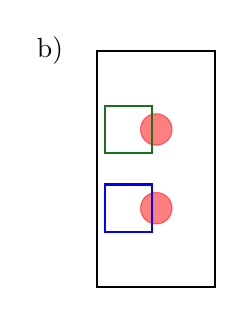
\begin{tikzpicture} 
        \node at (-0.6,3) {b)};
        \draw[thick] (0,0) rectangle (1.5,3);
        \draw[red,opacity=0.5, fill] (0.75,2) circle (0.2);   % pattern1
        \draw[red,opacity=0.5, fill] (0.75,1) circle (0.2);   % pattern1

        % readout windows
        \draw[thick,darkgreen] (0.1,1.7) rectangle (0.7,2.3);
        \draw[thick,blue] (0.1,0.7) rectangle (0.7,1.3);
      \end{tikzpicture} 
    };

    % Box 3: Stare
    \node[at={($(scope2.east)+(.6cm,0)$)},anchor=west](scope3){
      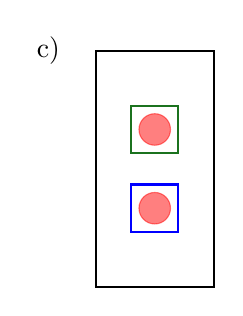
\begin{tikzpicture} 
        \node at (-0.6,3) {c)};
        \draw[thick] (0,0) rectangle (1.5,3);
        \draw[red,opacity=0.5, fill] (0.75,2) circle (0.2);   % pattern1
        \draw[red,opacity=0.5, fill] (0.75,1) circle (0.2);   % pattern1

        % readout windows
        \draw[thick,darkgreen] (0.45,1.7) rectangle (1.05,2.3);
        \draw[thick,blue] (0.45,0.7) rectangle (1.05,1.3);

      \end{tikzpicture} 
    };

    % Box 4: Move again
    \node[at={($(scope3.east)+(.6cm,0)$)},anchor=west](scope4){
      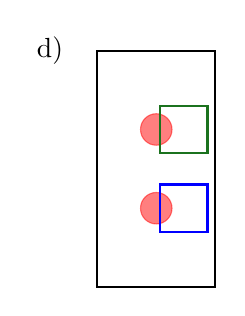
\begin{tikzpicture} 
        \node at (-0.6,3) {d)};
        \draw[thick] (0,0) rectangle (1.5,3);
        \draw[red,opacity=0.5, fill] (0.75,2) circle (0.2);   % pattern1
        \draw[red,opacity=0.5, fill] (0.75,1) circle (0.2);   % pattern1

        % readout windows
        \draw[thick,darkgreen] (0.8,1.7) rectangle (1.4,2.3);
        \draw[thick,blue] (0.8,0.7) rectangle (1.4,1.3);

      \end{tikzpicture} 
    };

    % Box 5: Readout 
    \node[at={($(scope4.east)+(.6cm,0)$)},anchor=west](scope5){
      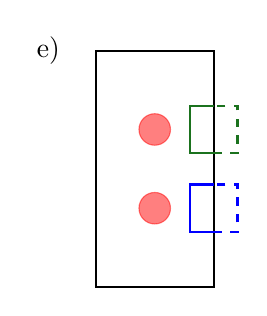
\begin{tikzpicture} 
        \node at (-0.6,3) {e)};
        \draw[thick] (0,0) rectangle (1.5,3);
        \draw[red,opacity=0.5, fill] (0.75,2) circle (0.2);   % pattern1
        \draw[red,opacity=0.5, fill] (0.75,1) circle (0.2);   % pattern1

        % readout windows
        \draw[thick,darkgreen,dashed] (1.5,1.7) -- (1.8,1.7) -- (1.8,2.3) -- (1.5,2.3);
        \draw[thick,darkgreen] (1.5,1.7) -- (1.2,1.7) -- (1.2,2.3) -- (1.5,2.3);

        \draw[thick,blue,dashed] (1.5,0.7) -- (1.8,0.7) -- (1.8,1.3) -- (1.5,1.3);
        \draw[thick,blue] (1.5,0.7) -- (1.2,0.7) -- (1.2,1.3) -- (1.5,1.3);

      \end{tikzpicture} 
    };

  \end{tikzpicture}
  \caption{Readout scheme for a BAM pattern. BAM fringe patterns are outlined as red circles. a) Create the readout windows. b) Move the readout windows via TDI. c) Stare observation -- charges are not shifted. d) Move readout windows via TDI. e) Readout, recording only contents of windows.}
  \label{fig:BAM_Acq}
\end{figure}

The observation principle and the effect on imaging particle tracks is shown in Fig. \ref{fig:BAM_Acq}. Effectively, data is collected from two windows, outlined in green and blue. These two windows have an unbinned length of 1000 in AL and 320 in AC each. They first move across the chip, stay in place during the staring, and then move again to the readout register.

The exposure can once again be viewed in two pictures, the physical pixel and image pixel based ones. In the former, it is easy to see that the entire region both readout windows cross are exposed -- the exposed area is 4500 $\times$ 320 pixels (AL $\times$ AC) per pattern. The exposure time, however, is more complex: First, the entire exposed region is exposed for $1000 T_\mathrm{TDI}$, due to the movement of the readout windows across the chip. Additionally, the region used for staring is observed for a further 19 s. The exposure time is, as such, AL-dependent.

In the image picture, the calculation is much easier. Viewing each readout window as a physical unit, the exposed area per window is simply 1000 $\times$ 320 pixels. The exposure time is simply the TDI transfer time plus the staring time.

The product of exposed area and exposure time, which is of interest for flux determination, is in both pictures

\begin{align}
  \mathrm{Physical: }~ A_\mathrm{exp} \cdot T_\mathrm{exp} = &2\left(4500 \cdot 10\,\mu m \cdot 320 \cdot 30\,\mu m \right) \cdot \left( 1000\, T_\mathrm{TDI} \right) \\+ &2\left( 1000 \cdot 10\,\mu m \cdot 320 \cdot 30\,\mu m\right) \cdot \left( 19\,s \right)\\
  \mathrm{Image: }~ A_\mathrm{exp} \cdot T_\mathrm{exp} = &2 \left( 1000 \cdot 10\,\mu m \cdot 320 \cdot 30\,\mu m\right) \cdot \left(4500\, T_\mathrm{TDI} + 19\,s \right)\\
  = &44.97\,\mathrm{cm^{2}\,s}
\end{align}

with the product of a single window obviously being half of this quantity.

As the computation is more simple in the image picture, we will from now on use this picture.

\section{Masked Pixels}

In both SM and BAM images, some image pixels can not be used for the determination of cosmics. In the SM, these pixels are mostly caused by the presence of bright stars, which saturate the CCDs. Transfer and overflow effects cause pixels that can be misidentified as cosmics or are on the whole useless for extracting cosmic rays. For the BAM, similar overflow effects can be caused by a high energy cosmics coincident with an interference fringe.

Correcting the exposed area for these masked pixels is very easy in the image picture, as we simply discard these pixels, meaning one can calculate the exposed area using

\begin{equation}
  A_\mathrm{exp} = (N_\mathrm{tot} - N_\mathrm{mask}) \cdot b_\mathrm{AL} \cdot b_\mathrm{AC} \cdot 10 \cdot 30 \, \mu m^{2}
\end{equation}

With $N_\mathrm{tot}$ being the total number of image pixels, $N_\mathrm{mask}$ being the number of masked pixels and $b_\mathrm{AL}$ and $b_\mathrm{AC}$ being the binning factor in AL and AC, respectively.
\end{document}
